% BEGIN LICENSE BLOCK
% Version: CMPL 1.1
%
% The contents of this file are subject to the Cisco-style Mozilla Public
% License Version 1.1 (the "License"); you may not use this file except
% in compliance with the License.  You may obtain a copy of the License
% at www.eclipse-clp.org/license.
% 
% Software distributed under the License is distributed on an "AS IS"
% basis, WITHOUT WARRANTY OF ANY KIND, either express or implied.  See
% the License for the specific language governing rights and limitations
% under the License. 
% 
% The Original Code is  The ECLiPSe Constraint Logic Programming System. 
% The Initial Developer of the Original Code is  Cisco Systems, Inc. 
% Portions created by the Initial Developer are
% Copyright (C) 2006 Cisco Systems, Inc.  All Rights Reserved.
% 
% Contributor(s): 
% 
% END LICENSE BLOCK

\newcommand{\jarlocation}{{\tt /lib/eclipse.jar}}
\newcommand{\docslocation}{{\tt /doc/javadoc/JavaEclipseInterface/index.html}}
\newcommand{\exampleslocation}{{\tt /doc/examples/JavaInterface}}

% Index entries
%
% classpath
% EclipseConnection interface
% EclipseEngine interface
% EmbeddedEclipse class
% RemoteEclipse class
% OutOfProcessEclipse class
% data types 
% equals() method
% rpc() method
% queues
% queues, opening
% queues, closing
% EXDR
% QueueListener interface




\chapter{Using the Java-{\eclipse} Interface}
\label{chapjava}
%HEVEA\cutdef[1]{section}
The Java-{\eclipse} Interface is a general-purpose tool for
interfacing {\eclipse} with Java, Sun's popular object-oriented
platform-independent programming language. It could be used for
example to write a Java graphical front-end to an {\eclipse} optimisation
program or to interface {\eclipse} with a commercial application
written in Java. This document assumes a moderate level of programming
in Java (e.g. how to use classes, packages, interfaces etc. and some
knowledge of the {\it java.util}, {\it java.io} and {\it java.net}
libraries) and a basic knowledge of how to interact with {\eclipse}
(e.g.\ how to execute a goal, nondeterminism, what lists are
etc.). There are also some diagrams in UML notation, but these are not
crucial to the reader's understanding.

Section \ref{sec:ji-getting-started} is intended to get you started
quickly by running the example program {\tt QuickTest.java}. Section
\ref{sec:ji-closer-look} gives a brief overview of the functionality
of the Java-{\eclipse} interface by taking a closer look at how {\tt
QuickTest.java} works. In the other sections of the document you will
learn how to write Java programs which can:
\begin{itemize}

\item Manipulate {\eclipse} terms and other data in Java (Section
\ref{sec:ji-terms-in-java}).
\item Execute goals in {\eclipse} and use the results of this
computation in Java (Section \ref{sec:ji-calling-goals}).
\item Transfer data between Java and {\eclipse} using queues\index{queues}.
(Section \ref{sec:ji-using-queue-streams}).
\item Initialise and terminate different kinds of connections between {\eclipse} and Java. (Section \ref{sec:ji-managing-eclipse-connections}).
\end{itemize}

Throughout this document, {\tt <eclipse\_dir>} stands for the root
location of your {\eclipse} installation. Detailed {\tt
javadoc}-generated HTML descriptions of the API provided by the {\tt
com.parctechnologies.eclipse} package can be found at:
\begin{quote}
\ahref{../javadoc/JavaEclipseInterface/index.html}{{\tt <eclipse\_dir>}\docslocation}
\end{quote}
You may wish to browse the API documentation after reading this
document to obtain more detailed descriptions of classes and
interfaces in the package.

\section{Getting Started}
\label{sec:ji-getting-started}
At the end of this section you will run the simple Java program {\tt
QuickTest.java} which uses {\eclipse}. First of all though
you need to check that your Java SDK version is recent enough and that
your classpath correctly set up.
\subsection{Check your Java SDK version}
Use of the Java-{\eclipse} Interface requires an installation of the
Java SDK (Standard Developer's Kit) version 1.2.2 or later. If your
Java SDK installation is an earlier version than this or you do not
have the Java SDK on your machine, the latest version can be
downloaded from Sun Microsystems Inc. (\ahrefurl{http://www.sun.com}).

\subsection{Make the {\tt com.parctechnologies.eclipse} package available in your class path}
The Java-{\eclipse} Interface consists mainly of a Java package which is
used as a library by the Java programs you will write. This package is
included as a {\tt .jar} file located within the {\eclipse} distribution at:
\begin{quote}
{\tt <eclipse\_dir>}\jarlocation
\end{quote}
You are free to copy {\tt eclipse.jar} to a more convenient
location. However, to compile or run any Java programs which use the
package you must include the full path of {\tt eclipse.jar} in your
classpath\index{classpath}. For more information on using the classpath, please consult
your Java documentation.

% this section no longer needed. 

%\subsection{Ensure that the libraries path is set correctly}
%During the operation of {\eclipse}, shared libraries/DLLs may need to
%be loaded dynamically. For this to occur, an environment variable 
%needs to be altered so that these are available. The details are
%platform-specific.

%\begin{itemize}
%\item On UNIX systems, the {\tt LD\_LIBRARY\_PATH}
%environment variable must include the path:
%\begin{quote}
%{\tt <eclipse\_dir>/lib/<architecture\_os>/}
%\end{quote}
%where {\tt <architecture\_os>} is for example {\tt i386\_linux} or 
%{\tt sparc\_sunos5}.
%\item On Windows operating systems, the {\tt PATH} environment variable must contain the path:
%\begin{quote}
%\begin{verbatim}
%<eclipse_dir>\lib\i386_nt\
%\end{verbatim}
%\end{quote}
%This setting should be made using the Windows Control
%Panel. Alternatively, the command starting the Java process can alter
%PATH before starting Java. Another option is to move the {\eclipse}
%DLLs to a system directory.
%\end{itemize}

\subsection{Compile and run {\tt QuickTest.java}}
\label{sec:ji-testing-ji}
To test that everything is working as it should be, and to see a quick
example of the Java-{\eclipse} Interface at work, try compiling and
running the Java program {\tt QuickTest.java}. This starts up an
{\eclipse} from Java and tells it to write a message to {\tt stdout}. The
program can be found at
\begin{quote}
\ahref{../examples/JavaInterface/QuickTest.java}{{\tt <eclipse\_dir>}\exampleslocation {\tt /QuickTest.java}}
\end{quote}

After compilation, to run the program, start the Java interpreter as
you normally would but before the name of the class, supply the
command line option
\begin{quote}
{\tt -Declipse.directory=<eclipse\_dir>}
\end{quote}
This tells Java where to find the {\eclipse} installation, so it can run
{\eclipse}. {\bf You should use this command line options when running
all other examples in this document}. When you run {\tt
QuickTest.java}, you should get a single line of output: {\tt hello
world}. How {\tt QuickTest.java} works is explained in Section
\ref{sec:ji-closer-look}.

\section{Functionality overview: A closer look at {\tt QuickTest.java}}
\label{sec:ji-closer-look}

To give a broad overview of how the Java-{\eclipse} Interface works,
we take a closer look at {\tt QuickTest.java}. Here is the Java source
code from {\tt QuickTest.java}.
\begin{verbatim}
import com.parctechnologies.eclipse.*;
import java.io.*;

public class QuickTest
{
  public static void main(String[] args) throws Exception
  {
    // Create some default Eclipse options
    EclipseEngineOptions eclipseEngineOptions = new EclipseEngineOptions();

    // Object representing the Eclipse engine
    EclipseEngine eclipse;

    // Connect the Eclipse's standard streams to the JVM's
    eclipseEngineOptions.setUseQueues(false);

    // Initialise Eclipse
    eclipse = EmbeddedEclipse.getInstance(eclipseEngineOptions);

    // Write a message
    eclipse.rpc("write(output, 'hello world'), flush(output)");

    // Destroy the Eclipse engine
    ((EmbeddedEclipse) eclipse).destroy();
  }
}

\end{verbatim}

The structure of the {\tt main} method in {\tt QuickTest.java}
contains elements which will appear in any Java code which uses the
Java-{\eclipse} interface. These are as follows:

\subsubsection*{Always import the {\tt com.parctechnologies.eclipse} package}
Note the first line using {\tt import}. We need to have this in every
Java source file which uses the Java-{\eclipse} Interface so that it can
load classes from the package.

\subsubsection*{Declare a reference to an {\it EclipseConnection} or an {\it EclipseEngine}}

{\it EclipseConnection} \index{EclipseConnection interface} and its
subinterface {\it EclipseEngine} \index{EclipseEngine interface} are Java
interfaces which contain the methods used when interacting with {\eclipse}.

\subsubsection*{Create an object which implements {\it EclipseConnection} or {\it EclipseEngine}}
There are a number of classes which implement these interfaces. In the case
of {\tt QuickTest.java} we use an instance of {\it EmbeddedEclipse}
\index{EmbeddedEclipse class}. The initialisation of these implementing
classes varies from class to class. In the case of {\it EmbeddedEclipse}
initialisation is done by creating and configuring an {\it
EclipseEngineOptions} object and using this in an invocation of the {\it
EmbeddedEclipse} class' static method {\tt getInstance}.

\subsubsection*{Interact with {\eclipse} using methods in the {\it EclipseConnection} or {\it EclipseEngine} interface}

We interact with the {\eclipse} engine by invoking methods on the object
which implements {\it EclipseConnection} \index{EclipseConnection
interface} or {\it EclipseEngine} \index{EclipseEngine interface}. In the
case of {\tt QuickTest.java} we invoke the {\tt rpc}\index{rpc() method} method, which causes
the {\eclipse} to execute a goal, in this case one which simply prints a
message.

\subsubsection*{Terminate interaction with the {\eclipse}}
In order to clean up, after the Java program has finished interacting
with {\eclipse}, the interaction should be terminated. Like
initialisation, how this termination is done varies among the classes
which implement the {\it EclipseConnection} and {\it EclipseEngine}
interfaces.  In the case of {\tt QuickTest.java}, termination is done
by invoking the {\tt destroy} method on the {\it EmbeddedEclipse}
object.\index{EmbeddedEclipse class}

\section{Java representation of {\eclipse} data}
\label{sec:ji-terms-in-java}
\index{{data types}, {Java}}
The Java-{\eclipse} Interface uses a set of conventions and Java classes so that data
types common in {\eclipse} can be represented. Representing {\eclipse} data types is useful for:
\begin{itemize}
\item Constructing compound goals to be sent to {\eclipse} for execution.
\item Deconstructing the results of {\eclipse}'s computation, which are returned as a compound goal.
\item Communicating compound terms and other data via queues\index{queues}. 
\end{itemize}
More details on these tasks will be provided in Sections
\ref{sec:ji-calling-goals} and \ref{sec:ji-using-queue-streams}, but it is first necessary to understand how {\eclipse} data is represented in Java.

\subsection{General correspondence between {\eclipse} and Java data types}
\label{sec:ji-type-correspondence}
Not all {\eclipse} data types are represented: for example, at present
the {\eclipse} type {\tt rational} has no Java equivalent. However, all
the most useful {\eclipse} types have a corresponding Java class.  Table
\ref{tab:ec-java-data} gives the general correspondence between those
{\eclipse} data types which are supported and the Java classes or
interfaces which are used to represent them. The {\eclipse} types/Java
classes which appear in the table are those which map to or from 
the {\eclipse} external data representation (EXDR)\index{EXDR} definition.

\begin{table}[htbp!]
\begin{center}
\begin{tabular}{|l|l|}
\hline 
{\eclipse} data type	 	& Java class/interface 		\\
\hline
{\tt atom}		& {\it Atom}			\\
\hline
{\tt compound} 		& {\it CompoundTerm}		\\
\hline
{\tt integer}		& {\it java.lang.Integer}	\\
			& {\it java.lang.Long}	\\
\hline
{\tt list}		& {\it java.util.Collection}	\\
\hline
{\tt float}		& {\it java.lang.Double}	\\
			& {\it java.lang.Float}		\\
\hline
{\tt string}		& {\it java.lang.String}	\\
\hline
{\tt variable}		& {\it null}	\\
\hline
\end{tabular}
\end{center}
\caption{\label{tab:ec-java-data}The correspondence between {\eclipse} and Java data types. The Java classes are within the {\tt com.parctechnologies.eclipse} package unless otherwise specified.} 
\end{table}
 

The general rule is that you can send data to {\eclipse} by passing
the relevant method an instance of the Java class corresponding to the
{\eclipse} data type you want on the {\eclipse} side. When data comes
back from {\eclipse} it will be an instance of {\it java.lang.Object}
but this can be cast to the relevant Java class, which must either be
known beforehand or determined e.g. using the {\tt getClass()} method.

There are also a number of peculiarities for certain cases which we
now explain.

\subsection{Atoms and compound terms}
\label{sec:ji-atoms-and-terms}
Atoms are simple: these are constructed in Java using the constructor
of the {\it Atom} class: the string parameter of the constructor
becomes the atom symbol. Although the Java interface {\it CompoundTerm} is
listed above, compound terms (except lists) are usually constructed
using the {\it CompoundTermImpl} class, which implements {\it
CompoundTerm}. Incidentally, {\it Atom} also implements {\it CompoundTerm}, even though strictly speaking {\eclipse} atoms are not compound. Here is an
example of {\it CompoundTermImpl} at work:

\begin{verbatim}
  // Construct a term in Java to represent the Eclipse term foo(a, b, 3).
  private static CompoundTerm construct_term()
  {
    Atom a = new Atom("a");
    Atom b = new Atom("b");
    Integer numberThree = new Integer(3);
    CompoundTerm theTerm = new CompoundTermImpl("foo", a, b, numberThree);

    return(theTerm);
  }
\end{verbatim}
This method is taken from the example Java program \ahref{../examples/JavaInterface/DataExample1.java}{{\tt DataExample1.java}}
which can be found in the examples directory {\tt
<eclipse\_dir>}\exampleslocation. The rest of the program sends
{\eclipse} a goal which tells it to write the term created by {\tt
construct\_term()} to {\tt stdout}.

In this example we use an {\it CompoundTermImpl} constructor whose
first parameter is a string which becomes the functor of the term. The
remaining parameters are instances of {\it java.lang.Object}. They may
be instances of any class or interface which appears in Table
\ref{tab:ec-java-data}. These become the arguments of the term. {\it
CompoundTermImpl} has a number of other convenient constructors. See
the API documentation for details of these.

Note that the object returned by {\tt construct\_term()} is declared
not as a {\it CompoundTermImpl} but as a {\it
CompoundTerm}. CompoundTerm is the Java interface for objects
representing compound terms. Anything which implements CompoundTerm
can be sent to {\eclipse} as a compound term.

Instead of using {\it CompoundTermImpl}, you may wish to implement
{\it CompoundTerm} yourself. The benefit of this is that you can pass
any object implementing {\it CompoundTerm} to an {\tt rpc}\index{rpc() method} invocation, and
it can supply a functor and arguments without the unnecessary creation
of another object. To do this you may wish to subclass {\it
AbstractCompoundTerm}.

\subsection{Lists}

Whenever you want to construct a list for {\eclipse} or deconstruct a
list coming from {\eclipse}, you use the {\it java.util.Collection}
interface. Look at the following method, taken from the example Java
program \ahref{../examples/JavaInterface/DataExample2.java}{{\tt DataExample2.java}} (which can be found in the examples
directory {\tt <eclipse\_dir>}\exampleslocation).

\begin{verbatim}
  // Construct a collection in Java to represent the Eclipse 
  // list [1, foo(3.5), bar].
  private static Collection construct_collection()
  {
      Collection theCollection = new LinkedList();

      theCollection.add(new Integer(1));
      theCollection.add(new CompoundTermImpl("foo", new Double(3.5)));
      theCollection.add(new Atom("bar"));

      return(theCollection);
  }
\end{verbatim}

If you study, compile and run {\tt DataExample2.java} you will see
that the collection is indeed translated into the required {\eclipse}
list. You will also see that order is maintained in the sense that the
order of elements as they appear in the {\eclipse} list will equal the
collection's iterator order (the converse is true if the data is
coming from {\eclipse} to Java).

Also note that the {\eclipse} empty list ({\tt []}) is represented in
Java by the constant {\it java.util.Collections.EMPTY\_LIST}.

\subsection{Floats and Doubles}

The {\eclipse} data type {\tt float} is always converted to {\it
java.lang.Double} in Java. However, {\eclipse} can be sent an instance
of {\it java.lang.Double} or {\it java.lang.Float}: both will be
converted to {\tt float} in {\eclipse}. One value of {\it
java.lang.Double} and {\it java.lang.Float} has no counterpart in
{\eclipse}: the not-a-number (NaN) value. Infinite values can be sent
in either direction.

\subsection{Integers}
{\eclipse} can be sent instances of either {\it java.lang.Integer}
(32-bit integers) or {\it java.lang.Long} (64-bit integers). Both of
these will be translated to type {\tt integer} on the {\eclipse} side.
When {\eclipse} sends data to Java, it will decide between the two
classes depending on the number of bits needed for the integer. So for
example, if the number is small enough to fit in an Integer, that is
what will be returned. Note that therefore, the type of number
coming back from {\eclipse} cannot be relied upon to be of one type or
the other if it could fall on either side of the 32-/64-bit boundary.

If you require a set of numbers coming from {\eclipse} to be all of
one Java type e.g. long, then the best approach is to cast the object
returned by {\eclipse} to an instance of {\it java.lang.Number} and
then invoke the appropriate conversion method e.g. {\tt longValue()}.

\subsection{Variables}
\label{sec:ji-variables-null}
The Java {\it null} token is used to represent any variables being
sent to {\eclipse}. All variables coming from {\eclipse} will appear as
{\it null}. The limitations of this are discussed in more detail in
Section \ref{sec:ji-calling-goals}.


\subsection{The {\tt equals()} method}
The {\tt equals()} method has been overridden for {\it
AbstractCompoundTerm} and therefore also for {\it Atom} and {\it
CompoundTermImpl}. The implementation returns {\tt true} iff the
parameter {\it Object} implements {\it CompoundTerm} and its functor
and arity are equal to those of the {\it AbstractCompoundTerm}, and
pairwise invocations of {\tt equals()} return {\tt true} between each
of the {\it AbstractCompoundTerm}'s arguments and the corresponding
argument of the parameter object.



\section{Executing an {\eclipse} goal from Java and processing the result}
\label{sec:ji-calling-goals}
The {\it EclipseConnection} \index{EclipseConnection interface} interface
provides a single method {\tt rpc}\index{rpc() method} (Remote Predicate Call) for executing
goals in the {\eclipse}. This method takes as a parameter the goal to be
executed. How to construct this parameter is dealt with in Section
\ref{sec:ji-rpc-parameter}. Section \ref{sec:ji-rpc-return} explains
how to deal with the results returned by {\tt rpc}\index{rpc() method}. Finally, some more
details about the execution of the goal are given in Section
\ref{sec:ji-goal-execution}. 

\subsection{Passing the goal parameter to {\tt rpc}\index{rpc() method}}
\label{sec:ji-rpc-parameter}
There are main two variants of {\tt rpc}\index{rpc() method} which differ in the class of the
goal parameter.

The simplest way to use {\tt rpc}\index{rpc() method} is to pass it an instance of {\it
java.lang.String} which should be the goal as it would be typed into
the {\eclipse} command line. Just like with the {\eclipse} command line,
the goal can be a conjunction of several subgoals. An example of this
is the use of {\tt rpc}\index{rpc() method} in the example program {\tt
QuickTest.java}. Also please note a full stop is not necessary.

The string-parameter {\tt rpc}\index{rpc() method} variant is somewhat inefficient and it
is also inflexible because creating goals dynamically, or goals
involving strings is tricky. It should really only be used for short
simple goals. A more flexible and efficient alternative is to invoke
{\tt rpc}\index{rpc() method}, passing it a parameter object which implements the {\it
CompoundTerm} interface (discussed in Section
\ref{sec:ji-atoms-and-terms}). In this case the term becomes the
goal. Here is an example of using this version of {\tt rpc}\index{rpc() method}, taken
from
\ahref{../examples/JavaInterface/DataExample1.java}{{\tt DataExample1.java}}.

\begin{verbatim}
    CompoundTerm a_term = construct_term();

    // Get Eclipse to write the term to stdout and flush 
    eclipse.rpc(
                new CompoundTermImpl(",",
                              new CompoundTermImpl("write", 
                                            new Atom("output"), a_term),
                              new CompoundTermImpl("flush", new Atom("output"))
                              )
                );
\end{verbatim}
Using this variant is a bit more cumbersome (e.g.\ the creation of a
new {\it CompoundTermImpl} for the conjunction of goals in the above
example) but it would be useful for large goals constructed
dynamically. There are also a number of ``convenience'' {\tt rpc}\index{rpc() method}
methods, where instead of providing a {\it CompoundTerm}, you provide
the objects from which the term is made. See the API documentation for
more details of these variants.

\subsection*{Note: \bipref{yield/2}{../bips/kernel/externals/yield-2.html}, \bipref{remote_yield/1}{../bips/kernel/externals/remote_yield-1.html} and {\tt rpc}\index{rpc() method}}

The builtins \bipref{yield/2}{../bips/kernel/externals/yield-2.html} and \bipref{remote_yield/1}{../bips/kernel/externals/remote_yield-1.html} should not be
executed anywhere within an {\tt rpc}\index{rpc() method} goal, as they will cause the
goal to return prematurely.

\subsection{Retrieving the results of an {\tt rpc}\index{rpc() method} goal execution}
\label{sec:ji-rpc-return}

The {\tt rpc}\index{rpc() method} method returns an object which implements {\it
CompoundTerm}. This object is the Java representation of the goal term, with
the solution substitution applied to its variables. 

The solution substitution can be deconstructed using the returned {\it
CompoundTerm}'s {\tt arg} method. This method takes an integer (the argument
position) and returns an Object which is the Java representation of
the {\eclipse} argument at that position.

In the returned {\it CompoundTerm} instantiated variables are replaced
with their instantiations. Hence even if the variable was named in the
initial goal, its instantiation is identified in the returned goal by
its {\it position} rather than its name. Uninstantiated variables in
the returned {\it CompoundTerm} are represented using the Java {\it null}
token.

If a variable in the {\tt rpc} goal becomes instantiated to an {\eclipse}
data type which does not have an equivalent EXDR type (such as breal), then
in the returned {\it CompoundTerm} it will appear as the Java {\it null}
token.

The following Java code is an example of how the returned {\it CompoundTerm}
can be deconstructed to extract the variable substitutions.
\begin{verbatim}
...
    CompoundTerm result = eclipse.rpc("X = Q, Y is 2.1 + 7");

    // The top-level functor of the goal term is ",". 
    // The first and second arguments of the goal term are the two subgoals
    // and we can safely cast these as CompoundTerms.
    CompoundTerm firstGoal = (CompoundTerm) result.arg(1);
    CompoundTerm secondGoal = (CompoundTerm) result.arg(2);
    // X is the first argument of the first goal.
    Object firstGoalFirstArg = firstGoal.arg(1);
    // Y is the first argument of the second goal.
    Object secondGoalFirstArg = secondGoal.arg(1);

    System.out.println("X = "+firstGoalFirstArg);
    System.out.println("Y = "+secondGoalFirstArg);
...
\end{verbatim}
The output will be:
\begin{verbatim}
X = null
Y = 9.1
\end{verbatim}
\subsubsection*{Other ways an {\tt rpc}\index{rpc() method} invocation can terminate}
Apart from succeeding and returning a {\it CompoundTerm}, {\tt rpc}\index{rpc() method} can throw
exceptions. If the goal fails, an instance of {\it Fail} is
thrown. So to test for failure you must catch this exception.  An
instance of {\it Throw} is thrown if {\eclipse} itself throws an
error.


\subsection{More details about {\tt rpc}\index{rpc() method} goal execution}
\label{sec:ji-goal-execution}
\subsubsection*{Variables}
As explained in Section \ref{sec:ji-variables-null}, {\eclipse}
variables are always represented by the {\it null} token, when {\tt
rpc}\index{rpc() method} is invoked with a {\it CompoundTerm} parameter. When used in an
{\tt rpc}\index{rpc() method} goal, each {\it null} token represents a different
variable. Using {\it CompoundTerm} you cannot represent a goal with
multiple occurrences of a single variable. So, for example the
following Java code will output {\tt q(b, b)} for the first {\tt rpc}\index{rpc() method}
invocation and {\tt q(a, b)} for the second.

\begin{verbatim}
...

  eclipse.rpc("assert(q(a, b))");
  eclipse.rpc("assert(q(b, b))");

  System.out.println(eclipse.rpc("q(X, X)"));
  System.out.println(eclipse.rpc(new CompoundTermImpl("q", null, null)));

...
\end{verbatim}

\subsubsection*{Nondeterminism}

The {\tt rpc}\index{rpc() method} feature does not support the handling of nondeterminism
in the execution of the {\eclipse} goal. If the goal succeeds, control
is returned to Java immediately after the first solution to the goal
is found in {\eclipse}. All choice-points thereafter are ignored. So,
for example, although the first {\eclipse} goal below would leave
choice-points, it would be equal in effect to the second.
\begin{verbatim}
...
result = eclipse.rpc("member(X, [1, 2, 3, 4, 5])");
...
result = eclipse.rpc("member(X, [1])");
\end{verbatim}
This is not a practical problem. It merely implies that if you are
using nondeterminism to generate multiple solutions, you should
collect these on the {\eclipse} side using a meta-level built-in
predicate such as {\tt findall/3} and then return the result to Java.

\subsubsection*{Concurrent invocations of {\tt rpc}\index{rpc() method}}

Note that the {\tt rpc}\index{rpc() method} method is {\tt synchronized}. Therefore if,
while one Java thread is currently executing an {\tt rpc}\index{rpc() method} invocation,
a second Java thread tries to invoke the {\tt rpc}\index{rpc() method} method of the same
{\it EclipseConnection}, the second thread will block until the first
thread's {\tt rpc}\index{rpc() method} invocation returns.

\subsubsection*{Nested invocations of {\tt rpc}\index{rpc() method}}

During the execution of the {\tt rpc}\index{rpc() method} method, control
 is transferred to {\eclipse}. Due to the {\it QueueListener} feature
 \index{QueueListener interface} which is discussed in Section
 \ref{sec:ji-using-queue-streams}, control is sometimes temporarily
 returned to Java before the {\eclipse} execution has finished. It is
 possible for this Java code itself to invoke {\tt rpc}\index{rpc()
 method}, thus leading to nested {\tt rpc}\index{rpc() method}
 invocations. Nested {\tt rpc}\index{rpc() method} invocations should not
 cause any problems.

\section{Communicating between Java and {\eclipse} using queues\index{queues}} 
\label{sec:ji-using-queue-streams}

In the Java-{\eclipse} Interface, {\it queues} are one-way data
streams used for communication between {\eclipse} and Java. These are
represented on the {\eclipse} side using ``peer queues'', which are 
I/O streams. The Java-{\eclipse} Interface includes the classes {\it
FromEclipseQueue} and {\it ToEclipseQueue} which represent these
queues on the Java side. {\it FromEclipseQueue} represents a queue
which can be written to in {\eclipse} and read from in Java. A {\it
ToEclipseQueue} is a queue which can be written to in Java and read
from in {\eclipse}.

Section \ref{sec:ji-open-close} discusses how queues are opened,
\index{queues, opening}referenced and closed\index{queues, closing} from either the Java 
or {\eclipse} sides. We also discuss here how to transfer byte data in both
directions. However, the programmer need not be concerned with low-level
data operations on queues: whole terms can be written and read using the
{\it EXDRInputStream} and {\it EXDROutputStream} classes discussed in
Section
\ref{sec:ji-formatting-queue-data}.

Via the {\it QueueListener} feature\index{QueueListener interface}, Java
code can be invoked (in a sense) from within {\eclipse}. The use of this
feature is discussed in Section \ref{sec:ji-queue-listeners}. In some
cases, the standard streams ({\tt stdin}, {\tt stdout} and {\tt stderr}) of
the {\eclipse} engine will be visible to Java as queues. How to use these
is discussed in Section \ref{sec:ji-standard-streams}.

\subsection{Opening, using and closing queues\index{queues}}
\label{sec:ji-open-close}
\index{queues, opening}
\index{queues, closing}
We now explain the standard sequence of events for using
queues. Opening and closing, can be performed in a single step from
either the Java or the {\eclipse} side.

\subsubsection*{Opening a queue using Java methods}

{\it FromEclipseQueue} and {\it ToEclipseQueue} do not have public
constructors. Instead, we invoke {\tt getFromEclipseQueue} or {\tt
getToEclipseQueue}. This asks the {\it EclipseConnection} object for a
reference to a {\it FromEclipseQueue} or {\it ToEclipseQueue} instance
which represents a new queue. To specify the stream for later
reference, we supply the method with a string which will equal to the
atom by which the queue is referred to as a stream in {\eclipse}. For
example the following code creates two queues\index{queues}, one in each direction:
\begin{verbatim}
...
  ToEclipseQueue java_to_eclipse = 
    eclipse.getToEclipseQueue("java_to_eclipse");
  FromEclipseQueue eclipse_to_java = 
    eclipse.getFromEclipseQueue("eclipse_to_java");
...
\end{verbatim}
These methods will create and return new {\it FromEclipseQueue} or
{\it ToEclipseQueue} objects, and will also open streams with the
specified names on the {\eclipse} side. No stream in {\eclipse} should
exist with the specified name. If a stream exists which has this name
and is not a queue between the Java object and {\eclipse}, the Java
method throws an exception. If the name is used by a pre-existing
queue, it is returned, so the {\tt getFromEclipseQueue} and {\tt
getToEclipseQueue} methods can also be used to retrieve the queue
objects by name once if they have already been created.

\subsection*{Opening a queue using {\eclipse} predicates}
\index{queues, opening}
You can use the {\eclipse} builtin \bipref{peer_queue_create/5}{../bips/kernel/externals/peer_queue_create-5.html} to open a
queue. Used correctly, these have the same effect as the Java methods
explained above. For the peer name, you should use the atom returned
by the {\tt getPeerName()} method of the relevant {\it
EclipseConnection} instance. The direction should be {\tt fromec} for
a {\it FromEclipseQueue} and {\tt toec} for a {\it
ToEclipseQueue}. The queue type should always be {\tt sync}
(for asynchronous queues, refer to section \ref{ji-async-queue-steams}).

\subsubsection*{Transferring data using Java methods}

On the Java side, once a {\it FromEclipseQueue} has been established,
you can treat it as you would any instance of {\it
java.io.InputStream}, of which {\it FromEclipseQueue} is a
subclass. Similarly, {\it ToEclipseQueue} is a subclass of {\it
java.io.OutputStream}. The only visible difference is that {\it
FromEclipseQueue} and {\it ToEclipseQueue} instances may have {\it
QueueListeners} attached, as is discussed in Section
\ref{sec:ji-queue-listeners}\index{QueueListener interface}. 

\subsubsection*{Transferring data using {\eclipse} predicates}

On the {\eclipse} side, there are built-in predicates for writing to,
reading from and otherwise interacting with streams. Any of these may
be used. Perhaps most useful are \bipref{read_exdr/2}{../bips/kernel/ioterm/read_exdr-2.html} and \bipref{write_exdr/2}{../bips/kernel/ioterm/write_exdr-2.html}; these are explained in Section
\ref{sec:ji-formatting-queue-data}\index{EXDR}. For the stream ID, you may either use the stream name, or the stream number, obtained for example using \bipref{peer_get_property/3}{../bips/kernel/externals/peer_get_property-3.html}.

\subsubsection*{Note: {\bf always} flush}

When communicating between Java and {\eclipse} using queues\index{queues}, you
should always invoke the {\tt flush()} method of the Java {\it
OutputStream} which you have written to, whether it be a {\it
ToEclipseQueue} or an {\it EXDROutputStream}. Similarly, on the
{\eclipse} side, {\tt flush/1} should always be executed after
writing. Although in some cases reading of the data is possible
without a flush, flushing guarantees the transfer of data.
% \footnote{Note that in extreme cases, even flushing a {\it
% ToEclipseQueue} does not guarantee that the data has been fully
% transferred to {\eclipse}: see Section \ref{sec:ji-toeclipse-remote}}

\subsubsection*{Closing a queue using Java methods}

This is done simply by calling the {\tt close()}\index{queues, closing} method on the {\it
FromEclipseQueue} or {\it ToEclipseQueue} instance.

\subsubsection*{Closing a queue using {\eclipse} predicates}
\index{queues, closing}
This is done by executing the builtin \bipref{peer_queue_close/1}{../bips/kernel/externals/peer_queue_close-1.html}. Note
that the builtin {\tt close/1} should not be used in this situation,
as it will not terminate the Java end of the queue.

\subsection{Writing and reading {\eclipse} terms on queues\index{queues}}
\label{sec:ji-formatting-queue-data}
Rather than dealing with low-level data I/O instructions such as reading
and writing bytes, the Java-{\eclipse} Interface provides classes for
reading and writing whole terms. In the underlying implementation of these
classes, the EXDR ({\eclipse} eXternal Data Representation) format is
used\index{EXDR}. This allows {\eclipse} to communicate with other
languages using a common data type. However, it is not necessary for the
API user to know about EXDR in detail to use the Java-{\eclipse} Interface
features discussed in this section.

{\it EXDRInputStream} is a subclass of {\it
java.io.DataInputStream} which can read EXDR format. {\it
EXDROutputStream} is a subclass of {\it
java.io.FilterOutputStream} which can write EXDR format.

\subsubsection*{Initialising {\it EXDRInputStream} and {\it EXDROutputStream}}
\index{EXDR}
The constructor for {\it EXDRInputStream} takes an instance of {\it
java.io.InputStream} as a parameter. This parameter stream is the
source of the EXDR data for the new stream. If data has been written
to the {\it InputStream} in EXDR format, you can access it by invoking
the {\tt readTerm} method of the new {\it EXDRInputStream}. This
will read the data from the {\it InputStream} and translate the EXDR
format into the Java representation of the data, which is then
returned by {\tt readTerm}.

Similarly, the constructor for {\it EXDROutputStream} takes an
instance of {\it java.io.OutputStream} as a parameter. This parameter
stream is the destination of the data written to the new stream. You
write data by invoking the {\tt write} method of the stream. The
parameter of this method is a Java object representing the piece of
data to be written. The class of this object can be any of the Java
classes mentioned in Table \ref{tab:ec-java-data}. The object gets
translated into EXDR format and this is written to the destination
{\it OutputStream}.

\subsubsection*{{\it EXDRInputStream} and {\it EXDROutputStream} at work}
\index{EXDR}
Although the underlying stream could be any kind of stream (e.g. a
file stream), the most common use of {\it EXDRInputStream} and {\it
EXDROutputStream} is to read data from and write data to queues\index{queues} in
EXDR format. In other words, we usually wrap these classes around {\it
FromEclipseQueue} and {\it ToEclipseQueue} classes. We now look at an
example which does just this.

The example is in these two files: 
\begin{quote}
\ahref{../examples/JavaInterface/QueueExample1.java}{{\tt <eclipse\_dir>}\exampleslocation {\tt /QueueExample1.java}}\\
\ahref{../examples/JavaInterface/queue\_example\_1.pl}{{\tt <eclipse\_dir>}\exampleslocation {\tt /queue\_example\_1.pl}}
\end{quote}
The Java program's first relevant action is to invoke the {\tt
compile} method of the {\it EclipseEngine}. This causes the {\eclipse}
program to be loaded by {\eclipse} engine. After {\tt compile}
completes, the Java program creates a {\it ToEclipseQueue} and a {\it
FromEclipseQueue}, with the following lines:
\begin{verbatim}
    // Create the two queues
    java_to_eclipse = eclipse.getToEclipseQueue("java_to_eclipse");
    eclipse_to_java = eclipse.getFromEclipseQueue("eclipse_to_java");
\end{verbatim}
Then in the next two lines we create an {\it EXDROutputStream} to
format data going to {\tt java\_to\_eclipse} and an {\it
EXDRInputStream} to format data coming from {\tt
eclipse\_to\_java}.
\begin{verbatim}
    // Set up the two formatting streams
    java_to_eclipse_formatted = new EXDROutputStream(java_to_eclipse);
    eclipse_to_java_formatted = new EXDRInputStream(eclipse_to_java);
\end{verbatim}
The Java program writes two atoms to {\tt
java\_to\_eclipse\_formatted}, and then flushes the stream. This
causes each atom to be translated into EXDR format and the translation
to then be written on to {\tt java_to_eclipse}. The Java program then
makes an {\tt rpc}\index{rpc() method} invocation to the {\eclipse} program's only predicate
{\tt read_2_write_1/0}, which is defined as follows:
\begin{verbatim}
read_2_write_1:-
        read_exdr(java_to_eclipse, Term1),
        read_exdr(java_to_eclipse, Term2),
        write_exdr(eclipse_to_java, pair(Term1, Term2)),
        flush(eclipse_to_java).
\end{verbatim}
The built-in \bipref{read_exdr/2}{../bips/kernel/ioterm/read_exdr-2.html} reads a term's worth of data from the
stream supplied and instantiates it to the second argument. So {\tt
read\_2\_write\_1/0} reads the two terms from the stream. They are
then written on to the {\tt eclipse\_to\_java} stream within a {\tt
pair(...)} functor using the built-in \bipref{write_exdr/2}{../bips/kernel/ioterm/write_exdr-2.html}, and the
stream is flushed. When the predicate succeeds, the {\tt rpc}\index{rpc() method} invocation
returns and the term data is on {\tt eclipse\_to\_java} in EXDR
format. The next step of the java program is the following:
\begin{verbatim}
    System.out.println(eclipse_to_java_formatted.readTerm());
\end{verbatim}
Since {\tt eclipse\_to\_java} was the {\it FromEclipseQueue} passed as a
parameter when {\tt eclipse\_to\_java\_formatted} was initialised, the
{\tt readTerm} method of this object reads the EXDR data which is on
{\tt eclipse\_to\_java} and converts it into the appropriate Object to
represent the piece of data, in this case a {\tt CompoundTerm}. This Object is
then returned by {\tt readTerm}. Hence the output of the program is
{\tt pair(a,b)}.

\subsection{Using the {\it QueueListener} interface}
\label{sec:ji-queue-listeners}
\index{QueueListener interface}
It may sometimes be useful to have Java react automatically to data
arriving on a queue from {\eclipse}. An example of this would
be where a Java program has a graphical display monitoring the state
of search in {\eclipse}. We would like {\eclipse} to be able to send a
message along a queue every time an element of the search state
updates, and have Java react with some appropriate graphical action
according to the message.

Similarly, {\eclipse} may require information from a Java database at
some point during its operation. Again we could use a queue to
transfer this information. If {\eclipse} tries to read from this queue
when it is empty, we would like Java to step in and supply the next
piece of data. 

The {\it QueueListener} interface is the means by which handlers are
attached to queues\index{queues} on the Java side so that Java reacts
automatically to {\eclipse}'s interaction with the queue.

Any object which implements the {\it QueueListener} interface can be
attached to either a {\it FromEclipseQueue} or a {\it ToEclipseQueue}, using
the {\tt setListener} method. The {\it QueueListener} can be removed
using {\tt removeListener}. Queues\index{Queues} can only have one Java
listener at any one time. 

The {\it QueueListener} interface has two methods: {\tt dataAvailable}
and {\tt dataRequest}. 

\begin{description}
\item[{\tt dataAvailable}] is invoked only if the {\it QueueListener} is 
  attached to a {\it FromEclipseQueue}. It is invoked when the queue is 
  flushed on the {\eclipse} side.
\item[{\tt dataRequest}] is invoked only if the {\it QueueListener} is 
  attached to a {\it ToEclipseQueue}. It is invoked when {\eclipse} tries
  to read from the queue when it is empty\footnote{Note that this invocation occurs only if the {\eclipse} side of the queue is empty. If you have written data to the queue on the Java side, but not flushed it, the {\eclipse} side may still be empty, in which case the {\tt dataRequest} method of the listener will be invoked.}.
\end{description}

Both methods have a single {\it Object} parameter named {\tt
source}. When they are invoked this parameter is the {\it FromEclipseQueue}
or {\it ToEclipseQueue} on which the flush or read happened.

There is an example Java program {\tt QueueExample2.java} with an
accompanying example {\eclipse} program {\tt queue\_example\_2.pl}
which use {\it QueueListeners} attached to queues going in both
directions.
\begin{quote}
\ahref{../examples/JavaInterface/QueueExample2.java}{{\tt <eclipse\_dir>}\exampleslocation {\tt /QueueExample2.java}}\\
\ahref{../examples/JavaInterface/queue\_example\_2.pl}{{\tt <eclipse\_dir>}\exampleslocation {\tt /queue\_example\_2.pl}}
\end{quote}
After the queues streams are set up on both sides, the Java program
attaches as listeners a {\it TermProducer} to the {\it ToEclipseQueue}
and a {\it TermConsumer} to the {\it FromEclipseQueue}. These are both
locally defined classes which implement {\it QueueListener}. The {\it
TermProducer}, each time its {\tt dataRequest} method is invoked, sends
one of five different atoms down its queue in EXDR format\index{EXDR}. The
{\it TermConsumer}, when its {\tt dataAvailable} method is invoked,
reads some EXDR data from its queue and translates it into the
appropriate Java object. It then writes this object out to stdout.

Next, the Java program, using {\tt rpc}\index{rpc() method}, executes the only predicate
in the {\eclipse} program: {\tt read\_5\_write\_5/0}. This repeats the
following operation five times: read in a term in EXDR format from the
relevant incoming stream, write it out in EXDR format with an
extra functor to the relevant outgoing stream, and flush the
outgoing stream.

\subsection{Access to {\eclipse}'s standard streams}
\label{sec:ji-standard-streams}
If the object representing the {\eclipse} implements the {\it
EclipseEngine} \index{EclipseEngine interface} interface, then the API user
may have access to the {\eclipse}'s standard streams (see Section
\ref{sec:ji-use-queues-flag}). These are returned as {\it
FromEclipseQueue}s and {\it ToEclipseQueue}s by the methods {\tt
getEclipseStdin}, {\tt getEclipseStdout} and {\tt getEclipseStderr}.

%%%%%%%%%%%%%%%%%%%%%%%%%%%%%%%%%%%%%%%%%%%%%%%%%%%%%%%%%%%%%%%%%%%%%%%%%%
\section{Asynchronous Communicating between Java and {\eclipse}\index{queues, asynchronous}} 
\label{sec:ji-async-queue-streams}

Starting with release 5.9, the {\it OutOfProcessEclipse}
and {\it RemoteEclipse} variants of the Java-{\eclipse} Interface also support
asynchronous queues through the class {\it AsyncEclipseQueue}\index{AsyncEclipseQueue}.
These are essentially socket connections between {\eclipse} and Java, which
can be used independently of which side has control. 

An {\it AsyncEclipseQueue} queue is opened and closed in the same way as 
a {\it FromEclipseQueue} or {\it ToEclipseQueue}, but the following
differences exist:
\begin{itemize}
\item an asynchronous queue can be read/written from the Java side
even while the ECLiPSe side has control, e.g. during an RPC.  This
obviously has to happen from a different thread than the one that
executes the RPC.
\item I/O operations on asynchronous queues can block, they should
therefore be done from a dedicated thread.
\item the AsyncEclipseQueue class does not extend InputStream or
OutputStream and can therefore not be used for I/O directly.  Instead,
a standard Java InputStream can be obtained from it via the
getInputStream() method, and an OutputStream via the getOutputStream()
method.
\item on the ECLiPSe side, an event can (and should) be raised when
data arrives from the Java side.  If the ECLiPSe side has control at
that time, it will handle the event.  Otherwise, the event handling
may be deferred until ECLiPSe has control back.
\end{itemize}

\subsection{Opening and closing asynchronous queues}
\label{sec:ji-async-open-close}
\index{queues, opening}
\index{queues, closing}
Opening and closing can be performed in a single step from
either the Java or the {\eclipse} side.

\subsubsection*{Opening an asychronous queue using Java methods}

The {\it AsyncEclipseQueue} does not have public
constructors. Instead, we invoke {\tt getAsyncEclipseQueue}.
This asks the {\it EclipseConnection} object for a
reference to an {\it AsyncEclipseQueue} instance
which represents a new queue. To specify the stream for later
reference, we supply the method with a string which will equal to the
atom by which the queue is referred to as a stream in {\eclipse}. For
example the following code creates such a queue\index{queues}:
\begin{verbatim} ...
  AsyncEclipseQueue java_eclipse_async = 
    eclipse.getAsyncEclipseQueue("java_eclipse_async");
...
\end{verbatim}
Note that this method will only work when the {\tt eclipse} object is
an {\it OutOfProcessEclipse} or {\it RemoteEclipse}.
Teh method will create and return a new {\it AsyncEclipseQueue}
object, and will also open a stream with the
specified names on the {\eclipse} side. No stream in {\eclipse} should
exist with the specified name. If a stream exists which has this name
and is not a queue between the Java object and {\eclipse}, the Java
method throws an exception. If the name is used by a pre-existing
queue, it is returned, so the {\tt getAsyncEclipseQueue}
methods can also be used to retrieve the queue
objects by name once they have already been created.

\subsection*{Opening an asychronous queue using {\eclipse} predicates}
\index{queues, opening}
You can use the {\eclipse} builtin \bipref{peer_queue_create/5}{../bips/kernel/externals/peer_queue_create-5.html} to open a
queue. Used correctly, these have the same effect as the Java methods
explained above. For the peer name, you should use the atom returned
by the {\tt getPeerName()} method of the relevant {\it
EclipseConnection} instance. The direction should be {\tt bidirect},
and the queue type should be specified as {\tt async}.

\subsubsection*{Transferring data using Java methods}

Once an {\it AsyncEclipseQueue} has been created, a standard Java
InputStream can be obtained from it via the getInputStream() method,
and an OutputStream via the getOutputStream() method.
These Java streams can be used as you would any instance of {\it
java.io.InputStream} or {\it java.io.OutputStream}.
Unlike the synchronous {\it FromEclipseQueue} and {\it ToEclipseQueue},
I/O on these streams can block, and should therefore be handled by dedicated
threads. For this reason, the listener-feature is not supported on
asynchronous queues.

\subsubsection*{Transferring data using {\eclipse} predicates}

On the {\eclipse} side, there are built-in predicates for writing to,
reading from and otherwise interacting with streams. Any of these may
be used. Perhaps most useful are \bipref{read_exdr/2}{../bips/kernel/ioterm/read_exdr-2.html} and \bipref{write_exdr/2}{../bips/kernel/ioterm/write_exdr-2.html}; these are explained in Section
\ref{sec:ji-formatting-queue-data}\index{EXDR}. For the stream ID, you may either use the stream name, or the stream number, obtained for example using \bipref{peer_get_property/3}{../bips/kernel/externals/peer_get_property-3.html}.

Since the {\eclipse} side does not support threads, it should only write to
an asynchronous queue when there is an active thread on the Java side to
read the data. Otherwise, the write-operation may block, and control will
never be transferred back from {\eclipse} to Java.

For reading from an asynchronous queue, the {\eclipse} side should
typically set up an event handler. The handler will be invoked whenever
new data arrives on a previously empty queue.
\begin{verbatim}
my_async_queue_handler(Stream) :-
    ( select([Stream], 0, [_]) ->
        read_exdr(Stream, Data),
        process(Data),
        my_async_queue_handler(Stream)
    ;
        events_nodefer
    ).

setup_async_queue_with_handler :-
    event_create(my_async_queue_handler(my_async_queue), [defers], Event),
    peer_queue_create(my_async_queue, host, async, bidirect, Event).
\end{verbatim}
Note that execution of the handler is only guaranteed when the {\eclipse}
side has control.

When communicating between Java and {\eclipse} using queues\index{queues}, you
should always invoke the {\tt flush()} method of the Java {\it
OutputStream} which you have written to, whether it be a {\it
ToEclipseQueue} or an {\it EXDROutputStream}. Similarly, on the
{\eclipse} side, {\tt flush/1} should always be executed after
writing. Although in some cases reading of the data is possible
without a flush, flushing guarantees the transfer of data.
% \footnote{Note that in extreme cases, even flushing a {\it
% ToEclipseQueue} does not guarantee that the data has been fully
% transferred to {\eclipse}: see Section \ref{sec:ji-toeclipse-remote}}

\subsubsection*{Closing a queue using Java methods}

This is done simply by calling the {\tt close()}\index{queues, closing} method on the {\it
AsyncEclipseQueue} instance.

\subsubsection*{Closing a queue using {\eclipse} predicates}
\index{queues, closing}
This is done by executing the builtin \bipref{peer_queue_close/1}{../bips/kernel/externals/peer_queue_close-1.html}. Note
that the builtin {\tt close/1} should not be used in this situation,
as it will not terminate the Java end of the queue.

\subsection{Writing and reading {\eclipse} terms on queues\index{queues}}
See the corresponding section for synchronous queues, 
\ref{sec:ji-formatting-queue-data}.

%%%%%%%%%%%%%%%%%%%%%%%%%%%%%%%%%%%%%%%%%%%%%%%%%%%%%%%%%%%%%%%%%%%%%%%%%%

\section{Managing connections to {\eclipse}}
\label{sec:ji-managing-eclipse-connections}
As of {\eclipse} 5.3 and later, there are three Java classes which can be
used to provide interaction with {\eclipse}. These are {\it
EmbeddedEclipse}\index{EmbeddedEclipse class}, {\it OutOfProcessEclipse}\index{OutOfProcessEclipse class}
and {\it RemoteEclipse}\index{RemoteEclipse class}. Although the three
classes all implement the {\it EclipseConnection} \index{EclipseConnection
interface} interface, there are some important differences in
initialisation, termination and use which are explained in this section. On
the {\eclipse} side, as of version 5.3 and later, there is a unified
interface for interaction with Java, based around the concept of a
`peer'. This is explained in Section
\ref{sec:ji-peer-concept}. Section
\ref{sec:ji-creating-eclipse-engines} discusses how to create an
{\eclipse} engine from within Java (this covers both {\it
EmbeddedEclipse} and {\it OutOfProcessEclipse}\index{OutOfProcessEclipse class}). Section
\ref{sec:ji-connecting-existing} discusses the {\it RemoteEclipse}
class, which allows Java to connect to an existing {\eclipse}
engine. Finally, Section \ref{sec:ji-compare-connection-classes}
compares the three connection classes, assessing the advantages and
disadvantages of each.

\subsection{A unified {\eclipse}-side interface to Java : the `peer' concept}
\label{sec:ji-peer-concept}

To allow {\eclipse} code to be independent of the way it is
interfacing with Java, there is a unified technique in {\eclipse} for
interfacing to Java and other non-{\eclipse} programs, based on the
concept of a {\it peer}. A peer is a computation environment which is
external to {\eclipse}, either in the sense of being a different
computer language or being a different process, possibly on a
different machine. When {\eclipse} is communicating with one or more
Java virtual machines using the Java-{\eclipse} interface (including
cases where {\eclipse} is embedded), it stores some global information
to keep track of each peer.

Each peer of the {\eclipse} engine is indexed within {\eclipse}
by a unique {\it peer name} which is an atom. This is set during the
initialisation of the connection between {\eclipse} and Java; the
details vary according to the Java class used to make the connection.

The peer name is used in those {\eclipse} predicate calls related to the
peer connection. In particular, those related to the opening and closing of
peer queues (see Section \ref{sec:ji-open-close}). The {\it
EclipseConnection} \index{EclipseConnection interface} interface includes
the method {\tt getPeerName()} which can be used to retrieve this name on
the Java side.

\subsection{Creating and managing {\eclipse} engines from Java}
\label{sec:ji-creating-eclipse-engines}

There are at present two options for creating an {\eclipse} engine from
Java. With {\it EmbeddedEclipse}\index{EmbeddedEclipse class}, the engine
takes the form of a dynamically loaded shared library within the Java
virtual machine. With {\it OutOfProcessEclipse}\index{OutOfProcessEclipse class} it is a separate, child
process of the Java virtual machine. These two options have in common that
they are both initialised using an {\it EclipseEngineOptions} object and
that both classes implement {\it EclipseEngine} \index{EclipseEngine
interface}.

\subsubsection{Configuring an {\it EclipseEngineOptions} object}
\label{sec:ji-eclipse-engine-options}
Before an {\eclipse} engine is created using either option, an {\it
EclipseEngineOptions} object must be created and configured. An
instance of the {\it EclipseEngineOptions} class represents our
configuration choices for a new {\eclipse} engine. 

The options can be specified by either looking them up in a {\it
java.util.Properties} instance or by calling ``set'' methods on the
{\it EclipseEngineOptions} instance.

In the first case you can either specify system properties (by passing
{\tt -D} command line options to the JVM) or you can use an {\it
EclipseEngineOptions} constructor which takes a {\it Properties}
parameter. Each option has a standard property name detailed below.

Once the {\it EclipseEngineOptions} object is created, there are
also ``set'' methods we can invoke on it to set the different options.

\begin{description}
\item [The {\eclipse} installation directory ({\tt
eclipse.directory})] This must be the correct path of an {\eclipse}
installation so that Java can find the files it needs to start
{\eclipse}. If an {\it EclipseEngineOptions} constructor is invoked
without a directory having been set, either using a constructor
parameter or as a property, an exception will be thrown.

\item [The default module ({\tt eclipse.default-module})] is the
default {\eclipse} module where goals are executed. If no setting is
made, then the default module will be ``eclipse''.

\item [Local and global size ({\tt eclipse.local-size} and {\tt eclipse.global-size})]
are the maximum size of the local stack and the global stack
respectively. In each case the option is an integer representing the
required size in megabytes. If no setting is made, the sizes default
to the {\eclipse} defaults.

\begin{description} 
\item [Local size] is the maximum combined size of the local 
  stack and the control stack. Roughly speaking, the local stack is
  the {\eclipse} equivalent of the call/return stack in procedural
  languages. The control stack is used to store the choicepoints which
  occur in the execution of non-deterministic code. You may therefore
  need to increase this limit if your search tree is exceptionally
  deep or if there is a lot of non-determinism. You can use the {\eclipse} goal
  {\tt get_flag(max_local_control, X)} to find out the current
  setting. For more details, see the section on ``Memory Organisation
  and Garbage Collection'' in the {\eclipse} User Manual.
\item [Global size] is the maximum combined size of the global 
  stack and the trail stack. The global stack is used to store data
  structures. The trail stack is used to store backtracking
  information and is therefore closely related to the control
  stack. You may need to increase this limit if you are creating large
  data structures in {\eclipse}, or if there is a lot of
  non-determinism. You can use the {\eclipse} goal {\tt
  get_flag(max_global_trail, X)} to find out the current
  setting. Again, see the section in the {\eclipse} User Manual for
  more details.
\end{description}

\item [The ``use queues'' flag ({\tt eclipse.use-queues})]
\label{sec:ji-use-queues-flag} If {\tt false} (the default case), the
{\eclipse} engine's standard streams ({\tt stdin}, {\tt stdout} and
{\tt stderr}) will be connected to the standard streams of the JVM. So
for example if, as in {\tt QuickTest.java}, a message is written to
{\tt stdout} from within {\eclipse}, this will appear on the {\tt
stdout} stream of the JVM. Similarly, if {\eclipse} requests input
from the {\tt stdin} stream, input will be requested from the {\tt
stdin} stream of the JVM. If the flag is set {\tt true}, {\it
FromEclipseQueue} and {\it ToEclipseQueue} objects are used to
represent the {\eclipse}'s standard streams.

\item [The peer name ({\tt eclipse.peer-name})] is the peer name by
which the Java side can be referenced within {\eclipse}, for example when
queues are created from the {\eclipse} side. By default the peer name for
the Java side when using an {\it EmbeddedEclipse}\index{EmbeddedEclipse
class} or an {\it OutOfProcessEclipse}\index{OutOfProcessEclipse class} is ``host''.

\end{description}

\subsubsection{Using {\it EmbeddedEclipse}}

\index{EmbeddedEclipse class}This section discusses issues specific to using the {\it
EmbeddedEclipse} class. With {\it EmbeddedEclipse}, the {\eclipse} engine
is a dynamically loaded native library in the Java virtual machine. Figure
\ref{fig:ji-embedded-deployment} shows this deployment model in UML
notation. The important consequences of this deployment model are:

\begin{itemize}
\item The {\eclipse} engine shares memory and other resources with Java. 
\item Only one such engine can exist in a Java virtual machine at any one time.
\item Communication between Java and {\eclipse} is very efficient.
\end{itemize}



% Now put the EPS file (generated from the original GIF file) into a figure

\begin{center}
  \begin{figure}[htb]
    \begin{center}
        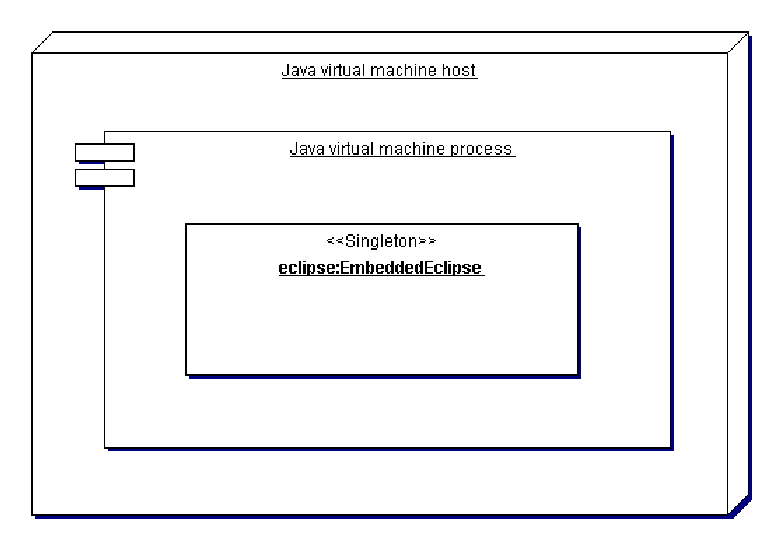
\includegraphics{embjava-diagrams/embedded-deployment.eps}
    \end{center}
    \caption{\label{fig:ji-embedded-deployment}UML deployment diagram for {\it EmbeddedEclipse}}
  \end{figure}
\end{center}



\paragraph{Initialising an {\it EmbeddedEclipse}}

The embedded {\eclipse} which runs within the JVM and shares its
resources, can be started and ended only once during the lifetime of
the JVM. There is no public constructor method for {\it
EmbeddedEclipse}. Initialisation of the embedded {\eclipse} is done
using the static {\tt getInstance} method of class {\it
EmbeddedEclipse} which takes an {\it EclipseEngineOptions} instance as
a parameter. The method uses this to configure and set up {\eclipse}
and then returns an object of type {\it EmbeddedEclipse}. There may
only ever be one instance of {\it EmbeddedEclipse} in a JVM. If the
embedded {\eclipse} has already been set up or if it has been set up
and terminated, subsequent invocations of {\tt getEclipse} with an
{\it EclipseEngineOptions} will throw exceptions. However during the
lifetime of the embedded {\eclipse}, a reference to the unique {\it
EmbeddedEclipse} object can be obtained using the parameterless static
{\tt getEclipse} method.

\paragraph{Termination of an {\it EmbeddedEclipse}}

The {\tt destroy} method which appears in the {\it EmbeddedEclipse}
class will shut the embedded {\eclipse} down. Once the {\tt destroy}
method has been invoked, the invocation of any methods which require
use of the {\eclipse} engine will result in an {\it
EclipseTerminatedException} being thrown. The {\tt destroy} method
should free all the resources of the JVM process which were being used
by the embedded {\eclipse}.

Once the {\it EmbeddedEclipse} has been destroyed, {\tt getEclipse}
can no longer be used during the lifetime of the JVM to initialise an
embedded {\eclipse} engine. In other words, by invoking {\tt destroy},
one removes the ability to use embedded {\eclipse} engines within the
current instance of the JVM.

\subsubsection{Using {\it OutOfProcessEclipse}\index{OutOfProcessEclipse class}}

This section discusses issues specific to the {\it
OutOfProcessEclipse}\index{OutOfProcessEclipse class} class.  With {\it OutOfProcessEclipse}, the
{\eclipse} engine is a child process of the Java virtual
machine. Figure \ref{fig:ji-outOfProcess-deployment} shows this deployment
model in UML notation. The important consequences of this deployment
model are:

\begin{itemize}
\item The {\eclipse} engine uses separate memory and other resources, 
depending on how the operating system allocates these between processes. 
\item Several instances of {\it OutOfProcessEclipse}\index{OutOfProcessEclipse class} can exist in a Java 
virtual machine at any one time.
\item Communication between Java and {\eclipse} is less efficient.
\end{itemize}

\begin{center}
  \begin{figure}[htb] 
  \begin{center} 
    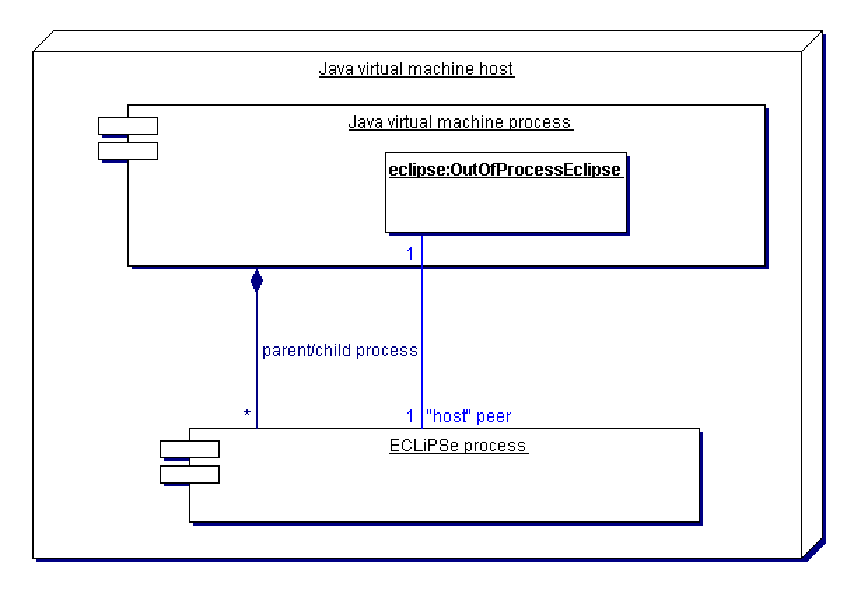
\includegraphics{embjava-diagrams/outOfProcess-deployment.eps}
  \end{center}
  \caption{\label{fig:ji-outOfProcess-deployment}UML deployment
    diagram for {\it OutOfProcessEclipse}} \end{figure}
\end{center}


\paragraph{Initialisation of an {\it OutOfProcessEclipse}\index{OutOfProcessEclipse class}}

{\it OutOfProcessEclipse}\index{OutOfProcessEclipse class} has a single constructor which takes an {\it
EclipseEngineOptions} object as its only parameter. See Section
\ref{sec:ji-eclipse-engine-options} for details of how to create and
configure this object. Unlike {\it EmbeddedEclipse}, multiple {\it
OutOfProcessEclipse}\index{OutOfProcessEclipse class} instances are allowed.

\paragraph{Termination of an {\it OutOfProcessEclipse}}

We invoke the instance method {\tt destroy()} in {\it
OutOfProcessEclipse}\index{OutOfProcessEclipse class} to terminate both the child {\eclipse} process
and our association with it. Once the {\tt destroy} method has been
invoked, the invocation of any methods on the destroyed {\it
OutOfProcessEclipse} object which require use of the {\eclipse} engine will
throw an {\it EclipseTerminatedException}. Unlike {\it
EmbeddedEclipse}, invoking {\tt destroy()} on an {\it
OutOfProcessEclipse} does not affect our ability to create new {\it
OutOfProcessEclipse} instances during the lifetime of the Java virtual
machine.

If the child process {\eclipse} crashes or is killed while {\eclipse}
has control, the Java thread which handed control to {\eclipse} should
throw an {\it EclipseTerminatedException}. If this happens while Java
has control, usually the next invocation of a method on the {\it
OutOfProcesEclipse} should throw an {\it EclipseTerminatedException},
although it is possible that some operations will throw a different
class of {\it IOException}. If this should happen it is worth calling
the {\tt destroy} method to do a final clean-up.

\subsection{Connecting to an existing {\eclipse} engine using {\it RemoteEclipse}\index{RemoteEclipse class}}
\label{sec:ji-connecting-existing}

In some applications, for example where Java is used to visualise
search in {\eclipse}, the life of the {\eclipse} engine may begin
before the connection with Java is initialised or end after the
connection with Java is terminated. Furthermore, it may also be useful
for the eclipse engine and the Java virtual machine to be running on
physically separate computers, for example if the {\eclipse} tasks are
being executed on a compute server, but the Java program is to be run
on a workstation. The {\it RemoteEclipse}\index{RemoteEclipse class} class can be used to connect
Java to {\eclipse} in these two scenarios. The deployment model is
that the {\it RemoteEclipse}\index{RemoteEclipse class} Java object is a ``Proxy'' for the
{\eclipse} engine which is running on the remote machine, as shown in
UML notation in Figure \ref{fig:ji-remote-deployment}.


\begin{center}
  \begin{figure}[htb]
    \begin{center}
        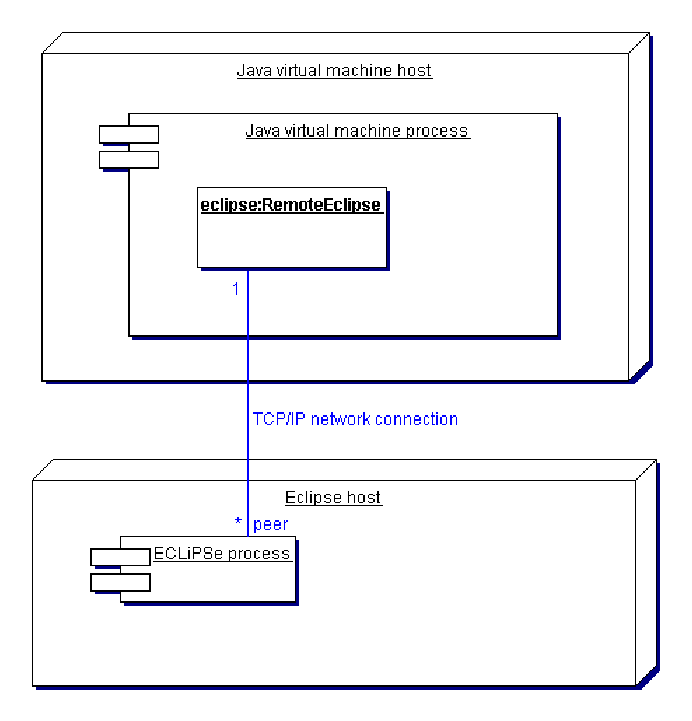
\includegraphics{embjava-diagrams/remote-deployment.eps}
    \end{center}
    \caption{\label{fig:ji-remote-deployment}UML deployment diagram for {\it RemoteEclipse}}
  \end{figure}
\end{center}

The key consequences of this deployment model are:
\begin{itemize}
\item {\eclipse} and Java can run on different machines and the two machines may have a different architecture/OS.  
\item {\eclipse} can connect to multiple Java processes using this model.
\item The lifetime of the {\eclipse} engine need not necessarily be a sub-duration of the lifetime of the JVM. 
\end{itemize}


\subsubsection{Initialisation of a {\it RemoteEclipse}\index{RemoteEclipse class} connection}
\label{sec:ji-remote-init}

Connecting Java to {\eclipse} using {\it RemoteEclipse} requires the
{\eclipse} engine to be primed so that it is ready to accept the
connection.  By the time it connects, the Java program must have the
IP address of the machine hosting the {\eclipse} engine (the server)
and the port number being used for the connection. The attachment
protocol also optionally allows for a password to be used by the Java
side and checked against one specified on the {\eclipse} side. Also
the server must be configured to allow TCP/IP socket servers which can
be connected to by the machine hosting Java. Initialising a connection
using {\it RemoteEclipse}\index{RemoteEclipse class} therefore requires some coordination between
the {\eclipse} code and the Java code. The Java code always consists
of a single {\it RemoteEclipse} constructor invocation, although the
constructor parameters may vary. 

The {\eclipse} side of the code uses certain builtins. Refer to the
relevant documentation of these for precise details of usage. On the
{\eclipse} side, the code can be structured in two different ways; one
simpler and the other allowing more flexibility. We outline here the
sequence of actions in each case.

\paragraph{Basic connection sequence}
This can be used in situations where no password is to be used and
where the port number is specified in advance, rather than generated
dynamically by {\eclipse}, and is known by the Java side.
\begin{enumerate}
  \item The {\eclipse} side executes the builtin \bipref{remote_connect/3}{../bips/kernel/externals/remote_connect-3.html}, specifying the port number in advance. This
	builtin will block until the connection is established.  

  \item The Java side then invokes one of the {\it RemoteEclipse}\index{RemoteEclipse class}
	constructors which has no password parameter. This should
	immediately complete or throw an exception if the connection
	is unsuccessful.

\end{enumerate}
\paragraph{Advanced connection sequence}
This more complicated sequence uses a password and optionally allows
the port number to be generated dynamically and then communicated to
the Java side.
\begin{enumerate}
  \item The {\eclipse} side executes the builtin \bipref{remote_connect_setup/3}{../bips/kernel/externals/remote_connect_setup-3.html}, specifying the password and either
	specifying the port number or allowing it to be generated
	dynamically.

  \item The port number must be communicated to the Java side somehow,
  	e.g. manually, or via a file.

  \item The Java side then invokes one of the {\it RemoteEclipse}\index{RemoteEclipse class}
	constructors with a password parameter. This either blocks
	until the connection is successful or throws an exception.

  \item The {\eclipse} side executes the builtin \bipref{remote_connect_accept/6}{../bips/kernel/externals/remote_connect_accept-6.html}, specifying the password which the
  	Java should supply.

  \item The Java constructor invocation then completes, or throws an
	exception if the connection could not be made.
\end{enumerate}

% something about localhost
If left as a free variable, the {\tt Host} argument of either the \bipref{remote_connect/3}{../bips/kernel/externals/remote_connect-3.html} or \bipref{remote_connect_setup/3}{../bips/kernel/externals/remote_connect_setup-3.html} goal will become
instantiated to the IP address of the machine hosting
{\eclipse}. Another possibility is to call the goal with this argument
already instantiated to the atom {\tt localhost}. This will mean that
only client connections made by processes on the same machine and
using the loopback address will be accepted. With this usage, on the
Java side you should use invoke {\tt
InetAddress.getHostByName("localhost")}. Note that {\tt
InetAddress.getLocalHost()} will not work in this situation.

In both connection sequences, the peer name indexing the connection is
either specified or generated dynamically on the {\eclipse} side in
the \bipref{remote_connect/3}{../bips/kernel/externals/remote_connect-3.html} or \bipref{remote_connect_setup/3}{../bips/kernel/externals/remote_connect_setup-3.html} goal.

Once the connection has been established by one of the above
sequences, control initially rests with the Java side. Therefore the
{\eclipse} code which called the \bipref{remote_connect/3}{../bips/kernel/externals/remote_connect-3.html} goal or the
\bipref{remote_connect_accept/6}{../bips/kernel/externals/remote_connect_accept-6.html} goal blocks until the Java side
explicitly transfers control to {\eclipse} or disconnects.

\subsubsection{Explicit transfer of control between {\eclipse} and Java}
\label{sec:ji-remote-control-transfer}

As mentioned above, after the initial connection has been established,
Java has control by default. However, this may not be convenient. For
example, in the case of search visualisation, after the initialisation
of the visualisation client, we may prefer {\eclipse} to have control
by default, allowing control to pass to Java only on certain
occasions. Control can be explicitly passed from Java to {\eclipse} by
invoking the {\tt resume()} method on a {\it RemoteEclipse}\index{RemoteEclipse class}. In this
case the {\eclipse} code will resume execution after the last point where
it passed control to Java. For example, if {\tt resume()} is invoked
immediately after the {\it RemoteEclipse}\index{RemoteEclipse class} constructor completes,
{\eclipse} execution will resume at the point just after the call to
the \bipref{remote_connect/3}{../bips/kernel/externals/remote_connect-3.html} goal or the \bipref{remote_connect_accept/6}{../bips/kernel/externals/remote_connect_accept-6.html}
goal.

Control can be transferred to a Java peer using the \bipref{remote_yield/1}{../bips/kernel/externals/remote_yield-1.html}
builtin. In this case the Java thread which passed execution to
{\eclipse} will resume execution at the point where it blocked.

The {\tt resume()} method and the \bipref{remote_yield/1}{../bips/kernel/externals/remote_yield-1.html} builtin should be
used with care. An invocation of {\tt resume()} should be paired with
an execution of a \bipref{remote_yield/1}{../bips/kernel/externals/remote_yield-1.html} goal in most cases. In addition,
\bipref{remote_yield/1}{../bips/kernel/externals/remote_yield-1.html} should not be executed in any code executed as a
result of an {\tt rpc}\index{rpc() method} invocation and {\tt resume()} should not be
executed within the {\it QueueListener} methods {\tt dataAvailable()}
or {\tt dataRequest()}.

The {\tt resume()} method and the \bipref{remote_yield/1}{../bips/kernel/externals/remote_yield-1.html} builtin should
only be used when other techniques such as {\tt rpc}\index{rpc() method} are not suitable.

% section not required: the only situation where there are problems can
% never occur, since you cannot read from a closed stream.


% \subsubsection{Using {\it ToEclipseQueue} objects with a {\it RemoteEclipse}}
% \label{sec:ji-toeclipse-remote}
% 
% The {\it java.io} API documentation specifies that the contract of the
% {\tt flush()} method of an {\it OutputStream} is to indicate to the
% stream that, if there are any buffered bytes they should ``immediately
% be written to their destination''. Since {\it ToEclipseQueue} is a
% subclass of {\it OutputStream}, ideally the completion of the {\tt
% flush()} method should guarantee that the bytes have been transferred
% to the {\eclipse} side of the connection. 
% 
% Unfortunately, there is an {\eclipse} limitation preventing this: the
% {\eclipse} side has a limited and fixed buffer size. So, in the case
% of {\it RemoteEclipse}, if a large enough number of bytes are written
% to a {\it ToEclipseQueue} the {\tt flush()} method cannot guarantee
% that the bytes have been transferred. However, it makes a lesser
% guarantee, that the bytes will be transferred as soon as possible when
% space becomes available in the {\eclipse}-side buffer. This will
% happen when a read of the queue is executed on the {\eclipse}
% side. Meanwhile the bytes are buffered on the Java side. When it
% becomes possible, the transfer is done automatically in a separate
% Java thread from the one which invoked {\tt flush}, so the API user
% does not normally need to worry about this.
% 
% The only situation where this potentially causes a problem is where a
% large number of bytes have been written to the {\it ToEclipseQueue}
% which is then flushed and closed before a corresponding read is
% executed on the {\eclipse} side. Since closing the queue does not wait
% for all the bytes to be transferred, these bytes may be lost. This may
% be avoided simply by ensuring that the last {\eclipse}-side read
% occurs before the queue is closed.
%
 
\subsubsection{Termination of a {\it RemoteEclipse} connection}
\label{sec:ji-remote-disconnect}

A {\it RemoteEclipse}\index{RemoteEclipse class} connection between {\eclipse} and Java may be
terminated in different ways. Firstly, disconnection may be initiated
by either side. Secondly the disconnection may be either {\it
multilateral} or {\it unilateral}. Multilateral disconnection, the
preferred method, is where the side which has control initiates
disconnection. Unilateral disconnection is where the side which
initiates disconnection does not have control, and should only take
place as a clean-up routine when one side is forced to terminate the
connection because of an unexpected event.


\begin{description}
 \item[Java-initiated multilateral disconnect] is performed by
 invoking the {\tt disconnect} method on the {\it RemoteEclipse}\index{RemoteEclipse class}
 instance while the Java side has control.

 \item[Java-initiated unilateral disconnect] is performed by
 invoking the {\tt unilateralDisconnect} method on the {\it
 RemoteEclipse}\index{RemoteEclipse class} instance while Java does not have control.

 \item[{\eclipse}-initiated multilateral disconnect] is performed on
 the {\eclipse} side by executing a \bipref{remote_disconnect/1}{../bips/kernel/externals/remote_disconnect-1.html} goal
 while {\eclipse} has control, identifying the connection to be closed
 by supplying the peer name.

 \item[{\eclipse}-initiated unilateral disconnect] cannot be
 executed by the user, since {\eclipse} is not
 multi-threaded. However, it may occur in certain urgent situations
 e.g. if the {\eclipse} process is killed while {\eclipse} does not
 have control.
\end{description}
If an {\eclipse}-initiated disconnect occurs, or the connection is
lost for whatever reason while {\eclipse} has control, the Java thread
which handed control to {\eclipse} should throw an {\it
EclipseTerminatedException}. If either of these happens while Java has
control, the next invocation of a method on the {\it
RemoteEclipse}\index{RemoteEclipse class} should throw an {\it EclipseTerminatedException},
although it is possible that some operations will throw a different
class of {\it IOException}. If this should happen it is worth invoking
the {\tt unilateralDisconnect()} method to do a final clean-up.

\subsection{Comparison of different Java-{\eclipse} connection techniques}
\label{sec:ji-compare-connection-classes}
This section should give you some idea of when it is most appropriate
to use each connection class. Figure \ref{fig:ji-connection-classes}
is a UML class diagram showing the most important relationships and
operations of the principal classes and interfaces. 

All three classes implement {\it EclipseConnection}
\index{EclipseConnection interface}, which provides all the functionality
you would expect during a ``session'' with {\eclipse}. The {\it
EclipseEngine} interface \index{EclipseEngine interface} is implemented
when the JVM ``owns'' the {\eclipse} engine, and so provides the methods to
access the standard I/O streams. Note that the termination methods are not
in either of the interfaces, but are specific to each class. Furthermore,
the {\tt resume()} method allows {\it RemoteEclipse}\index{RemoteEclipse class} to explicitly hand
control to {\eclipse}, but this operation is not supported by the other two
classes.

To summarise the advantages and disadvantages Table
\ref{tab:ji-feature-comparison} gives an at-a-glance comparison of the
different features of the different connection
classes.\index{EclipseConnection interface}\index{EclipseEngine interface}

\begin{center}
  \begin{figure}[htb]
    \begin{center}
        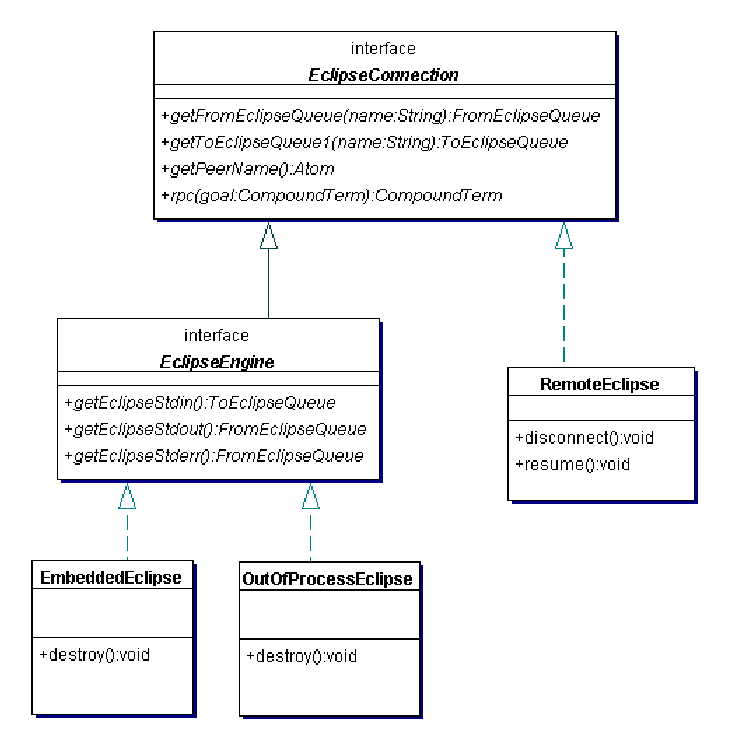
\includegraphics{embjava-diagrams/connection-classes.eps}
    \end{center}
    \caption{\label{fig:ji-connection-classes}UML class diagram for different classes connecting Java and {\eclipse}. Some convenience methods from {\it EclipseConnection} have been omitted.}
  \end{figure}
\end{center}


\begin{table}
\begin{center}
\begin{tabular}{|l|c|c|c|}
\hline
Feature			&\multicolumn{3}{|c|}{Java-{\eclipse} connection class}\\
\cline{2-4}
			&{\it Embedded}&{\it OutOfProcess}	&{\it Remote}\\
\hline
Implements {\it EclipseConnection} interface \ohtml{(allowing {\tt rpc}\index{rpc() method} and queues)}& $\bullet$ & $\bullet$ & $\bullet$\\
\olatex{(allowing {\tt rpc}\index{rpc() method} and queues) & & &\\}
\hline
Implements {\it EclipseEngine} interface \ohtml{(allowing access to {\eclipse} stdio streams)} & $\bullet$ & $\bullet$ & --\\
\olatex{(allowing access to {\eclipse} stdio streams) & & &\\}
\hline
{\eclipse} is in a separate process \ohtml{(with separate memory heap/stack)} & -- & $\bullet$ & $\bullet$ \\
\olatex{(with separate memory heap/stack) & & &\\}
\hline
{\eclipse} can be on a separate \ohtml{machine from Java}  & -- & -- & $\bullet$ \\
\olatex{machine from Java & & &\\}
\hline
{\eclipse} engine can start before/ \ohtml{end after Java virtual machine}  & -- & -- & $\bullet$ \\
\olatex{end after Java virtual machine & & &\\}
\hline
{\eclipse} engine created/ \ohtml{destroyed from Java}  & $\bullet$ & $\bullet$ & -- \\
\olatex{destroyed from Java & & &\\}
\hline
Efficient transfer of data on \ohtml{queues and {\tt rpc} invocations}  & $\bullet$ & -- & -- \\
\olatex{queues and {\tt rpc} invocations & & &\\}
\hline
One {\eclipse} can connect to many \ohtml{Java virtual machines using this}  & -- & -- & $\bullet$ \\
\olatex{Java virtual machines using this & & &\\}
\hline
One Java virtual machine can connect \ohtml{to many {\eclipse} engines using this}  & -- & $\bullet$ & $\bullet$ \\
\olatex{to many {\eclipse} engines using this & & &\\}
\hline
\end{tabular}
\end{center}
\caption{\label{tab:ji-feature-comparison} Feature comparison table for different {\eclipse} connection classes}
\end{table}

%HEVEA\cutend
 


